\documentclass{beamer}
\usepackage{amsmath}
\usepackage{graphicx}
\graphicspath{{./figures/}}

\usetheme{Boadilla}

\title{Introduction to Probabilities}
\author{Vasilis Gkolemis}
\institute{ATHENA RC | HUA}
\date{June 2025}

\begin{document}



\begin{frame}
  \titlepage
  \vfill
  \footnotesize
  \textcopyright\
  Vasilis Gkolemis, 2025. Licensed under CC BY 4.0.
\end{frame}

\section{Course Overview}

% one slide with the overview - six sessions (1 slide)

% one slide per session - discuss the topics (6 slides)


\begin{frame}{Helping Material}
  \begin{itemize}
    \item \textbf{Mathematics of Machine Learning} \url{https://mml-book.github.io/}
  \end{itemize}
\end{frame}


\section{The Role of Uncertainty in Machine Learning}

\subsection{Some motivational examples}

\begin{frame}{Variability}
\begin{itemize}
  \item Variability is part of nature.
  \item Data for 3 species of iris, from Ronald Fisher (1936).
\end{itemize}
\begin{center}
  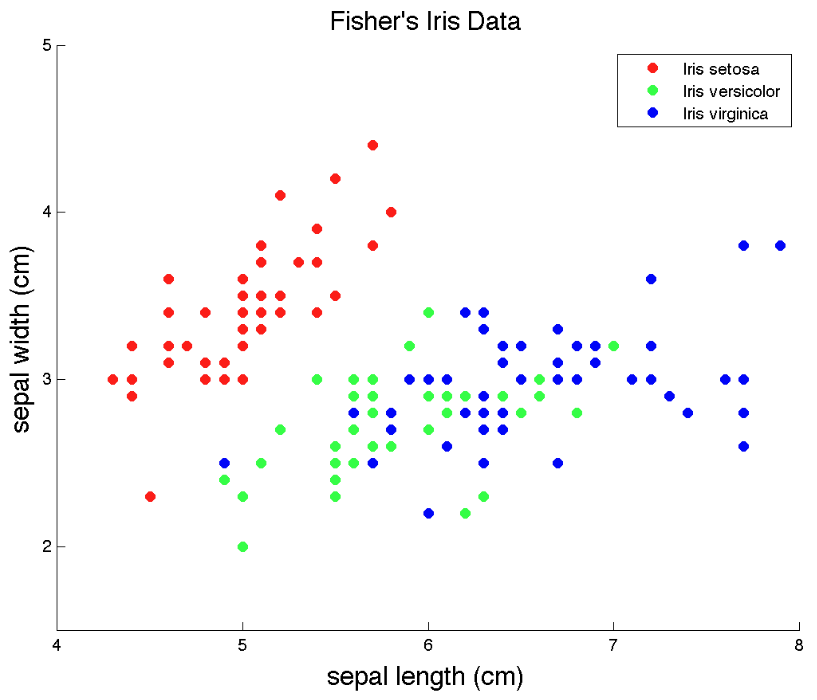
\includegraphics[width=0.6\textwidth]{iris_data.png}
\end{center}
\end{frame}

\begin{frame}{Variability}
\begin{itemize}
  \item Our handwriting is unique.
  \item Variability leads to uncertainty: e.g., distinguishing between 1 vs 7 or 4 vs 9.
\end{itemize}
\begin{center}
  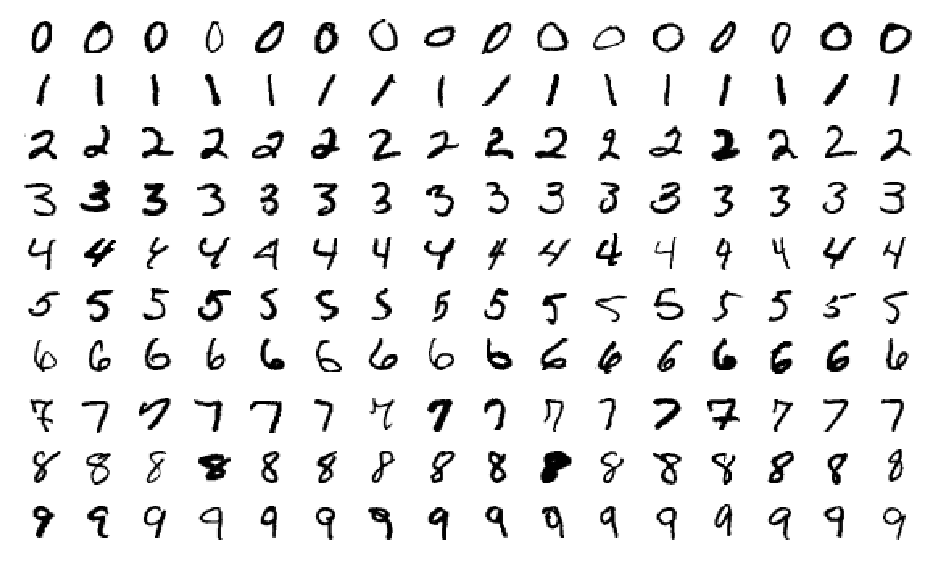
\includegraphics[width=0.6\textwidth]{handwriting_example.png}
\end{center}
\end{frame}

\begin{frame}{Variability}
\begin{itemize}
  \item Variability leads to uncertainty.
  \item Reading handwritten text in a foreign language.
\end{itemize}
\begin{center}
  
\includegraphics[width=0.5\textwidth]{foreign_handwriting.png}
\end{center}
\end{frame}

\begin{frame}{Example: Screening and Diagnostic Tests}
\begin{itemize}
  \item Early warning test for Alzheimer’s disease (Scharre, 2010, 2014).
  \item Detects “mild cognitive impairment”.
  \item Takes 10–15 minutes.
  \item Freely available.
  \item Assume a 70-year-old man tests positive.
  \item Should he be concerned?
\end{itemize}
\begin{center}
  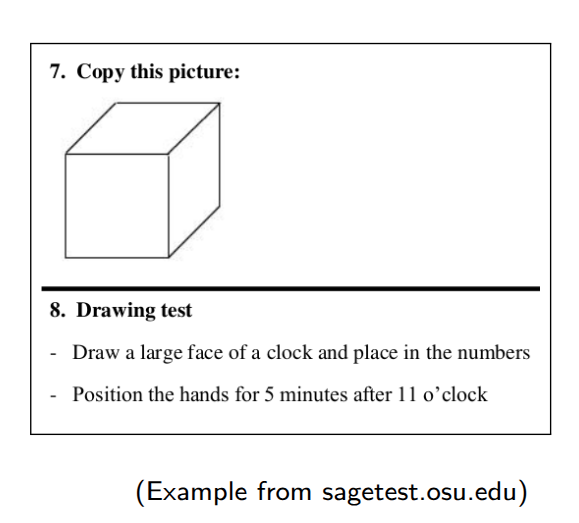
\includegraphics[width=0.4\textwidth]{sagetest_logo.png}
\end{center}
\end{frame}

\begin{frame}{Accuracy of the Test}
\begin{itemize}
  \item Sensitivity of 0.8 and specificity of 0.95 (Scharre, 2010).
  \item 80\% correct for people with impairment.
\end{itemize}
\begin{center}
  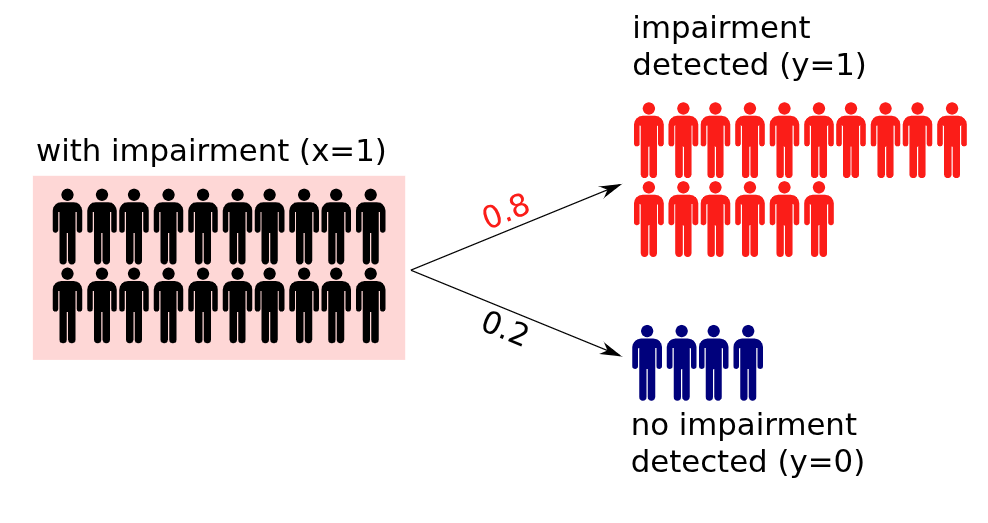
\includegraphics[width=0.8\textwidth]{with_impairment.png}
\end{center}
\end{frame}

\begin{frame}{Accuracy of the Test}
\begin{itemize}
  \item Sensitivity of 0.8 and specificity of 0.95 (Scharre, 2010).
  \item 95\% correct for people without impairment.
\end{itemize}
\begin{center}
  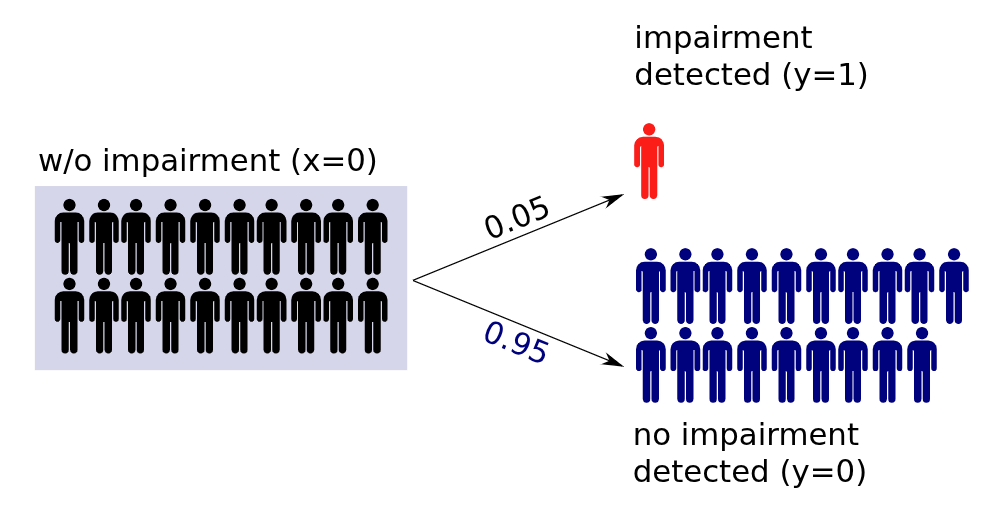
\includegraphics[width=0.8\textwidth]{without_impairment.png}
\end{center}
\end{frame}

\begin{frame}{Variability Implies Uncertainty}
\begin{itemize}
\item People of the same group do not have the same test results
  \begin{itemize}
  \item Test outcome is subject to variability.
  \item The data are noisy.
  \end{itemize}
\item Variability leads to uncertainty.
  \begin{itemize}
  \item Positive test $\equiv$ true positive?
  \item Positive test $\equiv$ false positive?
  \end{itemize}
\item What can we safely conclude from a positive test result?
\item How should we analyze such ambiguous data?
\end{itemize}
\end{frame}

\begin{frame}{Probabilistic Approach}
  \begin{itemize}
  \item $P(y\,|\,x)$: model of the test specified in terms of (conditional) probabilities.
  \item $x \in \{0, 1\}$: quantity of interest (cognitive impairment or not).
  \item $y \in \{0, 1\}$: test outcome (negative or positive).
  \item The test outcomes $y$ can be described with probabilities:
  \begin{itemize}
  \item Sensitivity = 0.8
    \begin{itemize}
    \item $\Rightarrow P(y = 1\,|\,x = 1) = 0.8$
    \item $\Rightarrow P(y = 0\,|\,x = 1) = 0.2$
    \end{itemize}
  \item Specificity = 0.95
    \begin{itemize}
    \item $\Rightarrow P(y = 0\,|\,x = 0) = 0.95$
    \item $\Rightarrow P(y = 1\,|\,x = 0) = 0.05$
    \end{itemize}
  \end{itemize}
\end{itemize}
\end{frame}


\begin{frame}{Prior Information}
\begin{itemize}
  \item Among people like the patient, $P(x = 1) = \frac{5}{45} \approx 11\%$ have a cognitive impairment (plausible range: 3\% – 22\%, Geda, 2014).
  \end{itemize}
  \begin{center}
    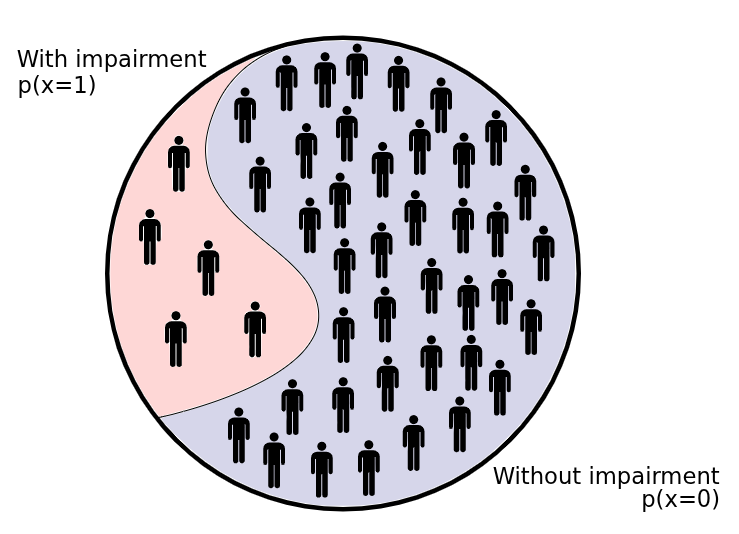
\includegraphics[width=0.7\textwidth]{prior.png}
  \end{center}
\end{frame}

\begin{frame}{Probabilistic Model}
\begin{itemize}
  \item Reality:
  \begin{itemize}
    \item Properties/characteristics of the group of people like the patient
    \item Properties/characteristics of the test
  \end{itemize}
\item Probabilistic model:
  \begin{itemize}
    \item $P(x = 1)$: probability of cognitive impairment
    \item $P(y = 1|x = 1)$ or $P(y = 0|x = 1)$: probability of positive or negative test given cognitive impairment
    \item $P(y = 1|x = 0)$ or $P(y = 0|x = 0)$: probability of positive or negative test given no cognitive impairment
  \item Fully specified by three numbers.
  \end{itemize}

  \item A probabilistic model is an abstraction of reality that uses probability theory to quantify the chance of uncertain events.
\end{itemize}
\end{frame}

\begin{frame}{If We Tested the Whole Population}
  \begin{center}
    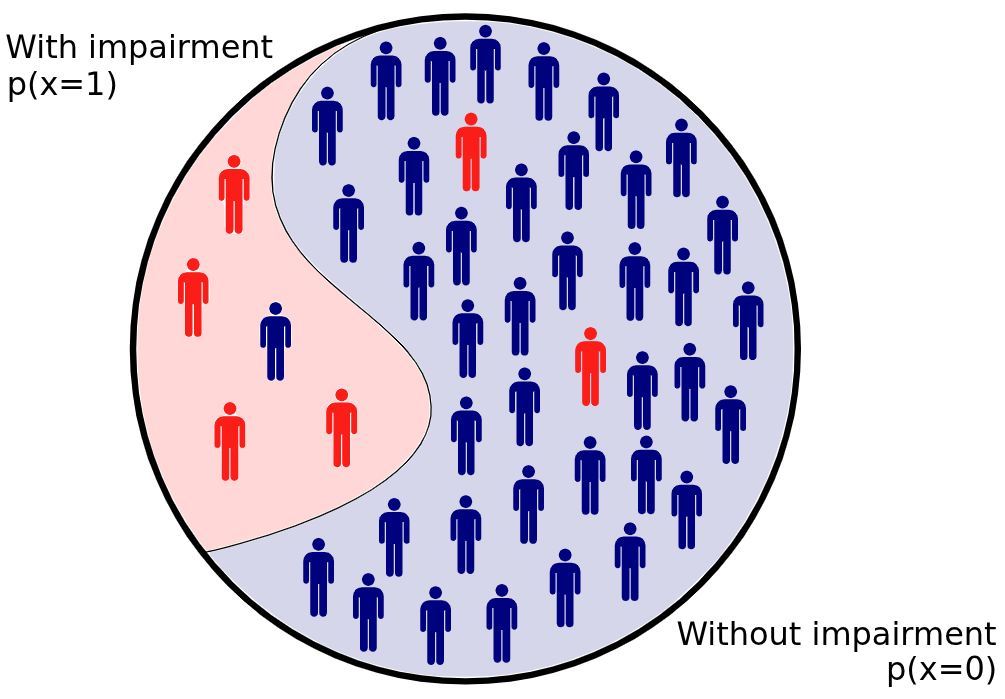
\includegraphics[width=0.8\textwidth]{whole_population.png}
  \end{center}
\end{frame}

\begin{frame}{If We Tested the Whole Population}
  \begin{itemize}
    \item Fraction of people who are impaired and test positive:
      \(
        P(x=1, y=1) = P(y = 1|x = 1)P(x = 1) = 0.8 \cdot \frac{5}{45} = \frac{4}{45} \approx 9\%
      \)
  \end{itemize}
  \begin{center}
    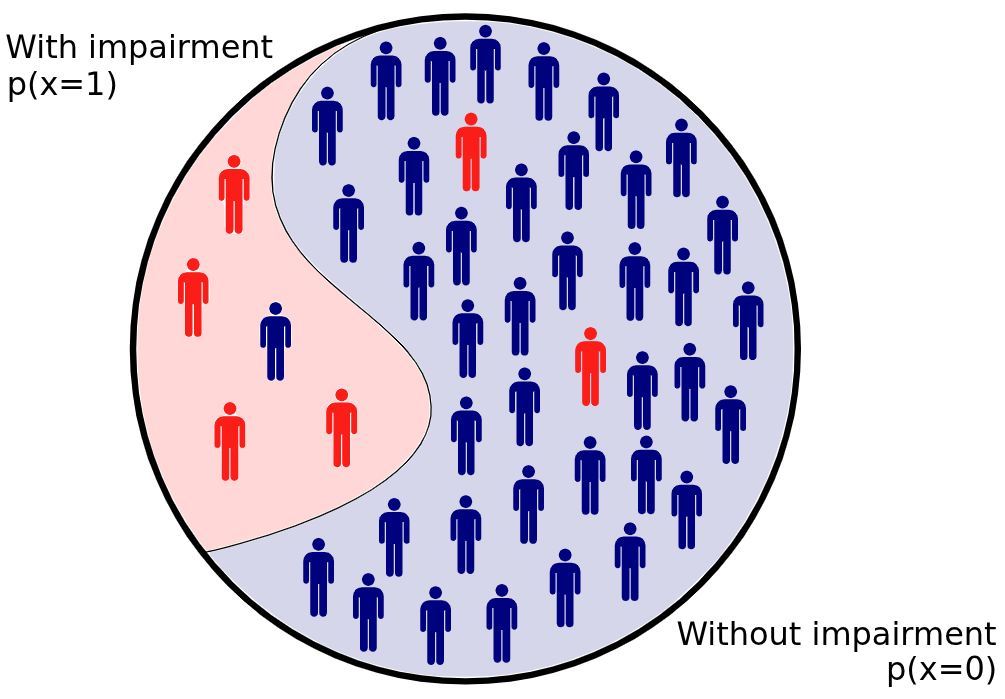
\includegraphics[width=0.7\textwidth]{whole_population.png}
  \end{center}
\end{frame}

\begin{frame}{If We Tested the Whole Population}
  \begin{itemize}
    \item Fraction of people who are not impaired and test positive:
      \(
        P(x=0, y=1) = P(y = 1|x = 0)P(x = 0) = 0.05 \cdot \frac{40}{45} = \frac{2}{45} \approx 4\%
      \)
  \end{itemize}
  \begin{center}
    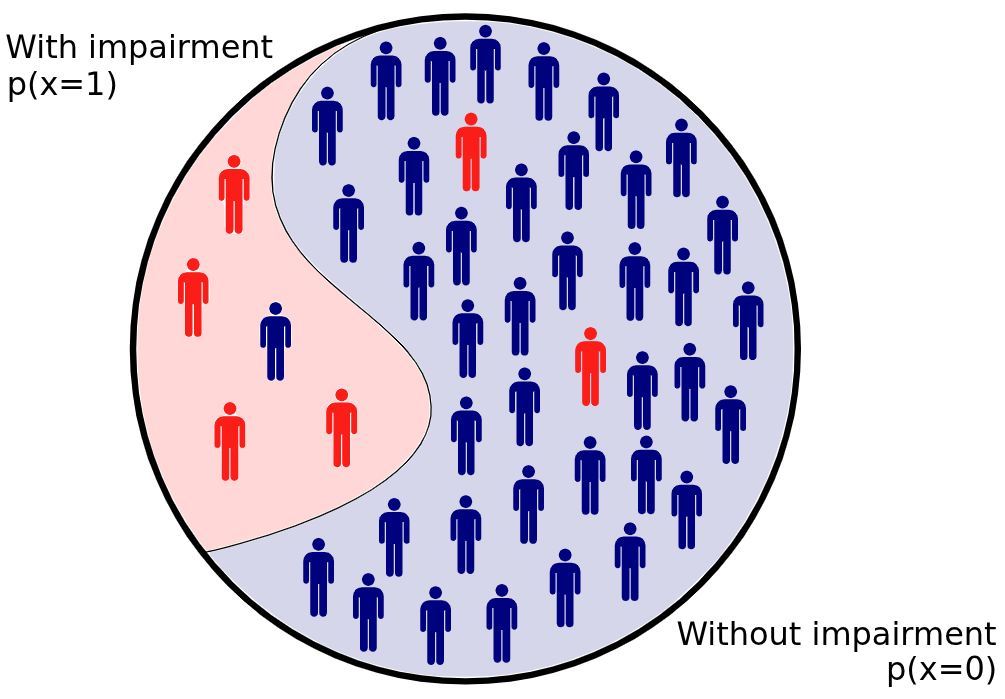
\includegraphics[width=0.7\textwidth]{whole_population.png}
  \end{center}
\end{frame}

\begin{frame}{If We Tested the Whole Population}
  \begin{itemize}
    \item Fraction of people where the test is positive:
      \(
        P(y=1) = P(x=1, y=1) + P(x=0, y=1) = \frac{4}{45} + \frac{2}{45} = \frac{6}{45} \approx 13\%
      \)
  \end{itemize}
  \begin{center}
    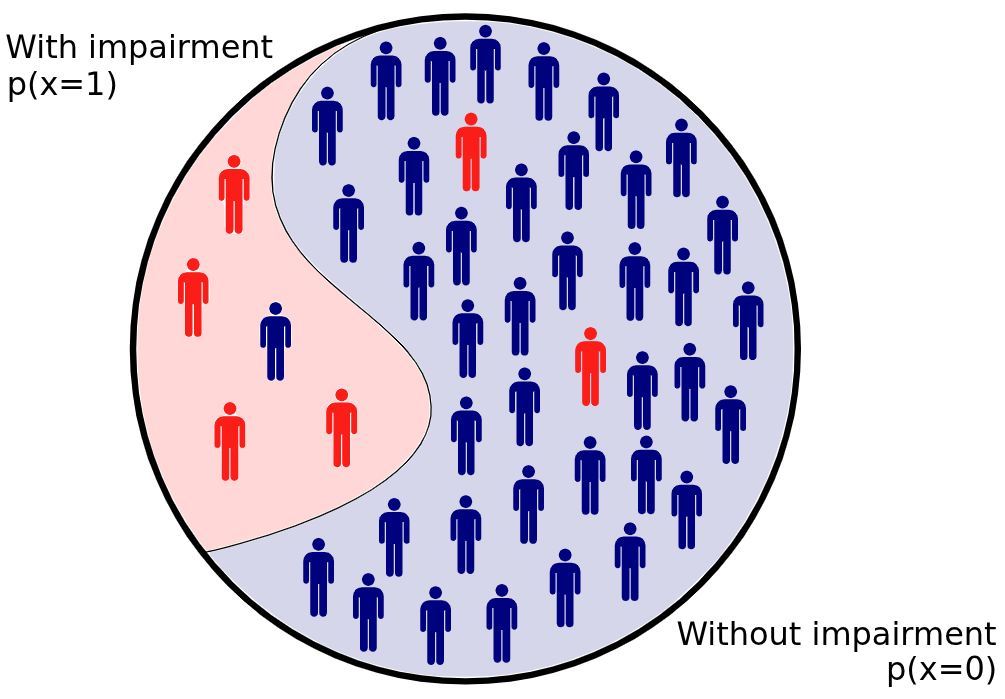
\includegraphics[width=0.7\textwidth]{whole_population.png}
  \end{center}
\end{frame}



\begin{frame}{Putting Everything Together}
\begin{itemize}
  \item Among those with a positive test, fraction with impairment:
  \[
  P(x = 1|y = 1) = \frac{P(y = 1|x = 1)P(x = 1)}{P(y = 1)} = \frac{4}{6} = \frac{2}{3}
  \]
  \item Fraction without impairment:
  \[
  P(x = 0|y = 1) = \frac{P(y = 1|x = 0)P(x = 0)}{P(y = 1)} = \frac{2}{6} = \frac{1}{3}
  \]
  \item Equations are examples of Bayes' rule.
  \item Positive test increased probability of cognitive impairment from $11\%$ (prior belief) to $67\%$, or from $6\%$ to $51\%$.
  \item $51\%$ (coin flip)
\end{itemize}
\end{frame}

\subsection{Probabilistic Modeling and Reasoning}

\begin{frame}{Probabilistic Modeling and Reasoning}
  \begin{itemize}
  \item Bayesian analysis is probabilistic modeling and reasoning using Bayes' rule.
  \item \textbf{Probabilistic modeling:}
    \begin{itemize}
      \item Model the world (events) using probabilities and random variables.
      \item Example random variables:
        \begin{itemize}
          \item $y$: test outcome
          \item $x$: cognitive impairment
        \end{itemize}
    \end{itemize}
  \item \textbf{Probabilistic reasoning (inference):}
    \begin{itemize}
      \item Compute probabilities of events given other events.
      \item Infer probabilities of unobserved events from observed data.
      \item Use \alert{Bayes' rule} to update beliefs based on evidence.
    \end{itemize}
\end{itemize}
\end{frame}

\begin{frame}{Probabilistic Modeling and Reasoning}
\begin{itemize}
  \item In our example:
    \begin{itemize}
      \item Unobserved/uncertain event: cognitive impairment $x = 1$
      \item Observed event (evidence): test result $y = 1$
      \item \textbf{Prior}: probability before seeing evidence, e.g., $P(x = 1)$
      \item \textbf{Posterior}: updated probability after evidence, e.g., $P(x = 1 | y = 1)$
    \end{itemize}
  \item \alert{Key idea:} The posterior quantifies what we believe about $x$ after seeing the test result $y$.
\end{itemize}
\end{frame}

\subsection{Key Rules of Probability}

\begin{frame}{Key Rules of Probability}
\begin{itemize}
\item \textbf{Product rule:}
  \begin{itemize}
    \item $P(x = 1, y = 1) = P(y = 1|x = 1)P(x = 1)$
    \item $P(x = 1, y = 1) = P(x = 1|y = 1)P(y = 1)$
  \end{itemize}
\item \textbf{Sum rule:}
  \begin{itemize}
  \item $P(y = 1) = P(x = 1, y = 1) + P(x = 0, y = 1)$
  \end{itemize}
\item \textbf{Bayes' rule (conditioning) as consequence of product rule:}
  \begin{itemize}
    \item $P(x = 1|y = 1) = \frac{P(x = 1, y = 1)}{P(y = 1)} = \frac{P(y = 1|x = 1)P(x = 1)}{P(y = 1)}$
  \end{itemize}
\item \textbf{Denominator from sum rule and product rule:}
  \begin{itemize}
    \item $P(y = 1) = P(y = 1|x = 1)P(x = 1) + P(y = 1|x = 0)P(x = 0)$
    \end{itemize}
\end{itemize}
\end{frame}

\begin{frame}{Key Rules of Probability}
  \begin{itemize}
  \item The rules generalize to multivariate random variables
    \begin{itemize}
      \item $\mathbf{x} = (x_1, x_2, \ldots)$: vector of random variables
      \item $\mathbf{y} = (y_1, y_2, \ldots)$: vector of random variables
      \end{itemize}
    \item The rules generalize to continuous random variables

    \item \textbf{Product rule:}
      \begin{itemize}
      \item $P(\mathbf{x}, \mathbf{y}) = P(\mathbf{y}|\mathbf{x})P(\mathbf{x})$
      \item $P(\mathbf{x}, \mathbf{y}) = P(\mathbf{x}|\mathbf{y})P(\mathbf{y})$
      \end{itemize}
    \item \textbf{Sum rule:}
      \begin{itemize}
      \item $P(\mathbf{y}) = \sum_{\mathbf{x}} P(\mathbf{x}, \mathbf{y})$ (discrete case)
      \item $P(\mathbf{y}) = \int P(\mathbf{x}, \mathbf{y}) d\mathbf{x}$ (continuous case)
      \end{itemize}
    \end{itemize}
\end{frame}

\section{Recap}

\begin{frame}{Recap}
  \begin{itemize}
    \item \textbf{Probabilistic Modeling:}
    \begin{itemize}
      \item The art of quantifying real-world phenomena with probabilities.
      \item Example: Diagnosing Alzheimer’s with a medical test.
    \end{itemize}

    \item \textbf{Probabilistic Reasoning (Inference):}
    \begin{itemize}
    \item Infer probabilites of unobserved events from observed data.
    \end{itemize}

    \item \textbf{Bayesian Analysis:}
      \begin{itemize}
      \item Bayes' rule updates our beliefs with new evidence.
      \item Applied in the Alzheimer’s test case.
    \end{itemize}

    \item \textbf{Core Probability Rules:}
    \begin{itemize}
      \item Product rule, Sum rule, Bayes' rule.
      \item These simple rules help us make informed conclusions.
    \end{itemize}
  \end{itemize}
\end{frame}

\begin{frame}{Recap \& What's Next}
\end{frame}


\end{document}
